\documentclass[11pt,a4paper]{article}
\input{reports/style}
\usepackage{tikz}
\usetikzlibrary{positioning,arrows.meta}
\renewcommand{\shorttitle}{Overview of all experiments}

\begin{document}
\reporttitle{Summary report}{Overview of All Experiments}{Seven experiments, 50,860 model answers, \$4.49}{30 October 2026}

\begin{plainabstract}
Anchoring is the tendency to be pulled towards a number you have just seen: asked whether Angel Falls is higher or lower than 11,000\,m, people (and models) then give higher estimates. This project asks \emph{why} language models anchor: do they start at the anchor and adjust away too little (\emph{adjusting}), or does the anchor bring matching facts to mind (\emph{retrieving})? So far we have run seven experiments on two models, a small one (R1-Distill-Qwen-1.5B) and a large one (Qwen3-32B), for \$4.49 in total. The first two tested the whole method. The small model was clearly anchored; the large model knew almost every answer and was hardly anchored at all, which taught us that anchoring needs uncertainty. We then screened 299 new questions and kept those the large model is unsure about. On these, the large model is anchored about as strongly as people (index 0.35--0.45; people about 0.49), and \textbf{letting it think longer does not reduce this}. The small model is anchored even more, often by copying the anchor. In Study~2, a starting value we \emph{give} the model pulls harder than one it thinks of \emph{itself}, in both models, as in people; but thinking helped the large model in both cases, so the strong human-based prediction was not supported. Read across all experiments, the anchor mostly works by changing what the model recalls, which points towards \emph{retrieving}. The next step is Qwen3-14B and a close reading of the large model's thinking.
\end{plainabstract}

\begin{keynumbers}
Experiments & 7 (two pilot runs, two screening rounds, Study~1, Study~2 on two models) \\
Answers & 50,860 (small test runs not counted) \\
Cost & \$4.49 on DeepInfra; the small model ran free on Colab \\
Models & R1-Distill-Qwen-1.5B (small, always thinks) and Qwen3-32B (large, thinking can be switched off) \\
Clearest findings & Anchoring needs uncertainty; on uncertain questions thinking does not reduce it in the large model; given values pull harder than own ones \\
Not run yet & Qwen3-14B on both studies (about \$3) \\
\end{keynumbers}

\section{The question}
Kahneman and Tversky showed that a number seen just before an estimate pulls the estimate towards it, even when the number is obviously irrelevant \citep{tversky1974judgment}. Psychology offers two explanations:
\begin{itemize}[leftmargin=*]
  \item \textbf{Adjusting:} people start at the anchor and move away step by step, stopping too early \citep{epley2006anchoring}.
  \item \textbf{Retrieving} (selective accessibility): the anchor makes facts that fit it come to mind, so the estimate is built from a biased set of memories \citep{mussweiler1999hypothesis}.
\end{itemize}
Language models anchor too \citep{lou2026anchoring}, and thinking longer does not reliably help. Models that write out their thinking let us watch which of the two processes happens. Two studies test this:
\begin{itemize}[leftmargin=*]
  \item \textbf{Study 1} gives an anchor in a \enquote{higher or lower than X?} question and varies its distance and precision. Adjusting predicts that answers stop near the edge of the plausible range; retrieving predicts that far anchors work no better than near ones.
  \item \textbf{Study 2} compares a starting value the model thinks of itself with the same value given to it. In people, effort helps only with self-generated starting values \citep{epley2005effortful}.
\end{itemize}

\section{The seven experiments}

\begin{figure}[ht]
\centering
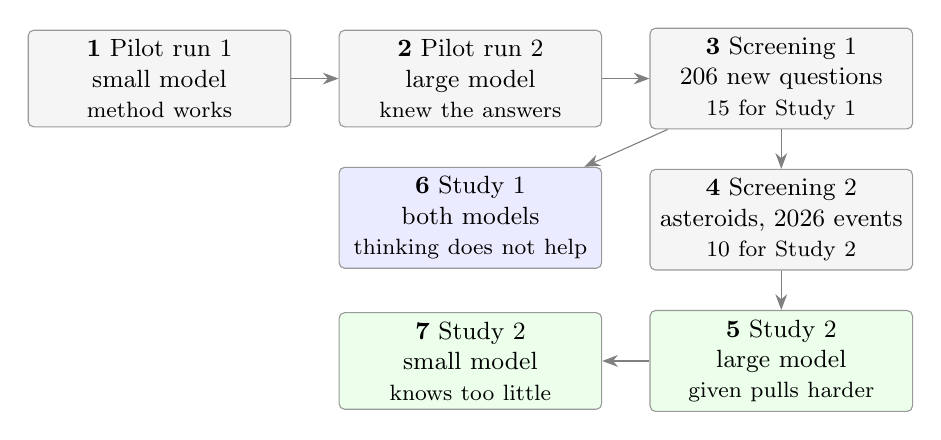
\begin{tikzpicture}[node distance=5mm and 6mm,
  box/.style={draw=black!40, rounded corners=2pt, fill=#1, align=center, font=\small, minimum height=12mm, text width=3.1cm},
  box/.default=black!4, arr/.style={-{Stealth[length=2mm]}, black!50}]
\node[box] (e1) {\textbf{1} Pilot run 1\\ small model\\ \footnotesize method works};
\node[box, right=of e1] (e2) {\textbf{2} Pilot run 2\\ large model\\ \footnotesize knew the answers};
\node[box, right=of e2] (e3) {\textbf{3} Screening 1\\ 206 new questions\\ \footnotesize 15 for Study 1};
\node[box, below=of e3] (e4) {\textbf{4} Screening 2\\ asteroids, 2026 events\\ \footnotesize 10 for Study 2};
\node[box=blue!8, below=of e2] (e6) {\textbf{6} Study 1\\ both models\\ \footnotesize thinking does not help};
\node[box=green!8, below=of e4] (e5) {\textbf{5} Study 2\\ large model\\ \footnotesize given pulls harder};
\node[box=green!8, left=of e5] (e7) {\textbf{7} Study 2\\ small model\\ \footnotesize knows too little};
\draw[arr] (e1) -- (e2); \draw[arr] (e2) -- (e3); \draw[arr] (e3) -- (e4);
\draw[arr] (e3) -- (e6); \draw[arr] (e4) -- (e5); \draw[arr] (e5) -- (e7);
\end{tikzpicture}
\caption{How the experiments led to each other. Blue: Study~1; green: Study~2.}
\label{fig:flow}
\end{figure}

\begin{table}[ht]
\centering\small
\begin{tabular}{@{}rp{4.2cm}p{3.3cm}rrl@{}}
\toprule
\# & Experiment & Model(s) & Answers & Cost & Report \\
\midrule
1 & Pilot run 1 (24 Oct) & R1-Distill-Qwen-1.5B & 7,200 & free & \texttt{exp1\_pilot\_run1} \\
2 & Pilot run 2 (26 Oct) & Qwen3-32B & 7,200 & \$1.52 & \texttt{exp2\_pilot\_run2} \\
3 & Screening, round 1 (26 Oct) & Qwen3-32B, 1.5B & 16,480 & \$0.97 & \texttt{exp3\_screening1} \\
4 & Screening, round 2 (26 Oct) & Qwen3-32B, 1.5B & 7,440 & \$0.44 & \texttt{exp4\_screening2} \\
5 & Study 2, large model (29 Oct) & Qwen3-32B & 1,800 & \$0.62 & \texttt{exp5\_study2} \\
6 & Study 1, new questions (30 Oct) & Qwen3-32B, 1.5B & 8,940 & \$0.94 & \texttt{exp6\_study1} \\
7 & Study 2, small model (30 Oct) & R1-Distill-Qwen-1.5B & 1,800 & free & \texttt{exp7\_study2\_small} \\
\midrule
 & Total & & 50,860 & \$4.49 & \\
\bottomrule
\end{tabular}
\caption{All experiments. Each has its own full report in this folder; short two-page versions are in \texttt{reports/short/}.}
\end{table}

\section{The story, one experiment at a time}

\paragraph{1. Pilot run 1: the method works, and the small model anchors.} 30 questions, 7,200 answers on a free Colab GPU. After a high anchor of 11,000\,m, the small model \enquote{remembered} Angel Falls as 11,700\,m tall (true 979\,m). Its anchoring index was 0.36--0.58, close to people. Reading 40 thinking traces showed the anchor acting at the moment a value was recalled; step-by-step adjustment appeared in only 1 of 40.

\paragraph{2. Pilot run 2: the large model knew the answers.} Qwen3-32B said 979\,m for Angel Falls in 238 of 240 anchored answers. Index 0.00--0.05. Where it was unsure, the anchor chose \emph{which memory} won: Liechtenstein's population as 39,000 or ten times that, 390,000; a high anchor raised the wrong memory from 30\% to 50\% of answers.

\paragraph{3. Screening round 1: finding what the model does not know.} 206 new questions, each asked 40 times without an anchor. The large model knew 94 of 137 Study~1 candidates; it was unsure about numbers it must estimate (windows of Versailles: answers from 1,300 to 14,000, true 2,143). 15 questions picked.

\paragraph{4. Screening round 2: questions for Study 2.} 54 asteroid orbits and 39 numbers from 2026 events. Bennu showed the ideal pattern: 366 days without thinking, 433 with Kepler's law (true 437). 10 questions picked where thinking moves the answer towards the truth.

\paragraph{5. Study 2 on the large model.} A given starting value pulled harder than the model's own at every thinking level (own 0.18 / 0.53 / 0.62 vs given 0.00 / 0.18 / 0.28 of the way to the truth). Thinking helped both, so the strong prediction failed. \enquote{Accuracy matters} helped the own version more in 9 of 9 questions, as in people.

\begin{figure}[ht]
\centering\rfig[0.8\textwidth]{ov_index}
\caption{Anchoring index for near anchors in every Study~1 run. Dashed: the original 30 questions (Experiments~1 and~2); solid: the 15 screened questions (Experiment~6). Orange: Qwen3-32B; blue: R1-Distill-Qwen-1.5B. On the original questions the large model was hardly anchored because it knew the answers; on the screened questions it is anchored about as much as people, at every thinking level.}
\label{fig:index}
\end{figure}

\paragraph{6. Study 1 on the new questions.} The key result of the project so far (Figure~\ref{fig:index}). On questions it is unsure about, the large model is anchored at a human level, 0.35--0.45, and short or long thinking does not reduce it. Its whole range of answers slides towards the anchor; it rarely copies. The small model is anchored more (up to 0.83) and copies the anchor in 15--25\% of answers, mostly when its thinking is cut off; longer thinking does help it (0.59).

\paragraph{7. Study 2 on the small model.} Again the given value pulled harder (repeated back in 24--26\% vs 10--16\% of answers), but only about a quarter of answers moved closer to the truth, so the main question cannot be answered on this model.


\section{What we know now}
\begin{enumerate}[leftmargin=*]
  \item \textbf{Anchoring needs uncertainty.} When a model knows the answer, the anchor does nothing (Experiment~2). On questions it is unsure about, the same model is anchored like people (Experiment~6).
  \item \textbf{Thinking longer does not fix anchoring in the large model.} This fits the 2026 report that bigger thinking budgets do not help, now on questions chosen to be uncertain.
  \item \textbf{A given number pulls harder than a self-generated one}, in both models, as in people.
  \item \textbf{Small and large models anchor differently.} The small one copies the anchor, especially when its thinking is cut off; the large one shifts its whole range of answers.
  \item \textbf{The evidence leans towards retrieving.} Anchors change which value is recalled (Angel Falls 11,700\,m, Liechtenstein's two memories); step-by-step adjustment is rare in traces. This still has to be tested properly on the large model's traces.
\end{enumerate}

\begin{cautionbox}[A correction, and honest limits.]
In Experiment~1 the small model with thinking off usually left out the \texttt{Estimate:} line, and the code took the last number in the reply, often the anchor repeated back. Read strictly (only replies with the line), its thinking-off index is 0.58, not 0.82. Every report now uses the strict reading. More generally: this is a pilot with two models and 10--15 questions per study; question-selection rules were set after seeing data; the thinking limits (512 and 2,048 tokens) cut off much of the thinking. These are reasons to treat the numbers as directions, not final values.
\end{cautionbox}

\section{Next steps}
\begin{enumerate}[leftmargin=*]
  \item \textbf{Run Qwen3-14B on both studies} (about \$3): a middle model of the same family, with a real \enquote{off} switch.
  \item \textbf{Read the large model's thinking traces} in Study~1: does it start at the anchor and adjust, or recall anchor-like facts? This is the mechanism question of the project.
  \item \textbf{Raise the thinking limits} (1,024 and 4,096 tokens) so that thinking finishes, and ask for the number only when thinking is off.
  \item \textbf{Add more Study~2 questions} of the asteroid and Mario-film kind, where the model really recalls the starting value.
\end{enumerate}

\appendix
\section{Where everything is}
\begin{itemize}[leftmargin=*]
  \item Full reports: \texttt{reports/exp1\_pilot\_run1.tex} to \texttt{reports/exp7\_study2\_small.tex}; short versions in \texttt{reports/short/}
  \item Longer earlier reports: \texttt{full\_report.tex} (up to 27 October), \texttt{pilot\_summary.tex},\\ \texttt{qwen3\_report.tex}, \texttt{events\_2026.tex} and \texttt{study2\_qwen3.tex}
  \item Code, notebooks and data: the GitHub repository (\texttt{data/}, \texttt{results/}, \texttt{notebooks/})
\end{itemize}

\bibliographystyle{plainnat}
\bibliography{references}
\end{document}
